\newcommand{\ts}{\textsuperscript}
\section{Exercise 4}
The purpose of this exercise to explore the connection between the singular
value decomposition (SVD) and face recognition. Start by downloading the
files \texttt{Faces.mat} and storing it locally in a directory
jupyter-notebook can read. The file contains the images of 38
different faces with 64 different lighting scenarios in which we will use
the first 36 faces to train our algorithm on and the last two to
demonstrate its potential. Next perform the following task:
\begin{enumerate}[label=\arabic*.]
    \item Download the pseudo code \texttt{Torres-SVD-face.py} and adjust
        the code so that it runs up to the section ``Plotting all the faces
        individually''. You may have to adjust the directory paths, and
        download \texttt{scipi}. Ensure the code is running correctly by
        plotting and displaying the figures for faces 8 and 24.
        \begin{mdframed}[style=MyFrame]
            The following are faces 8 and 24:
            \begin{figure}[H]
                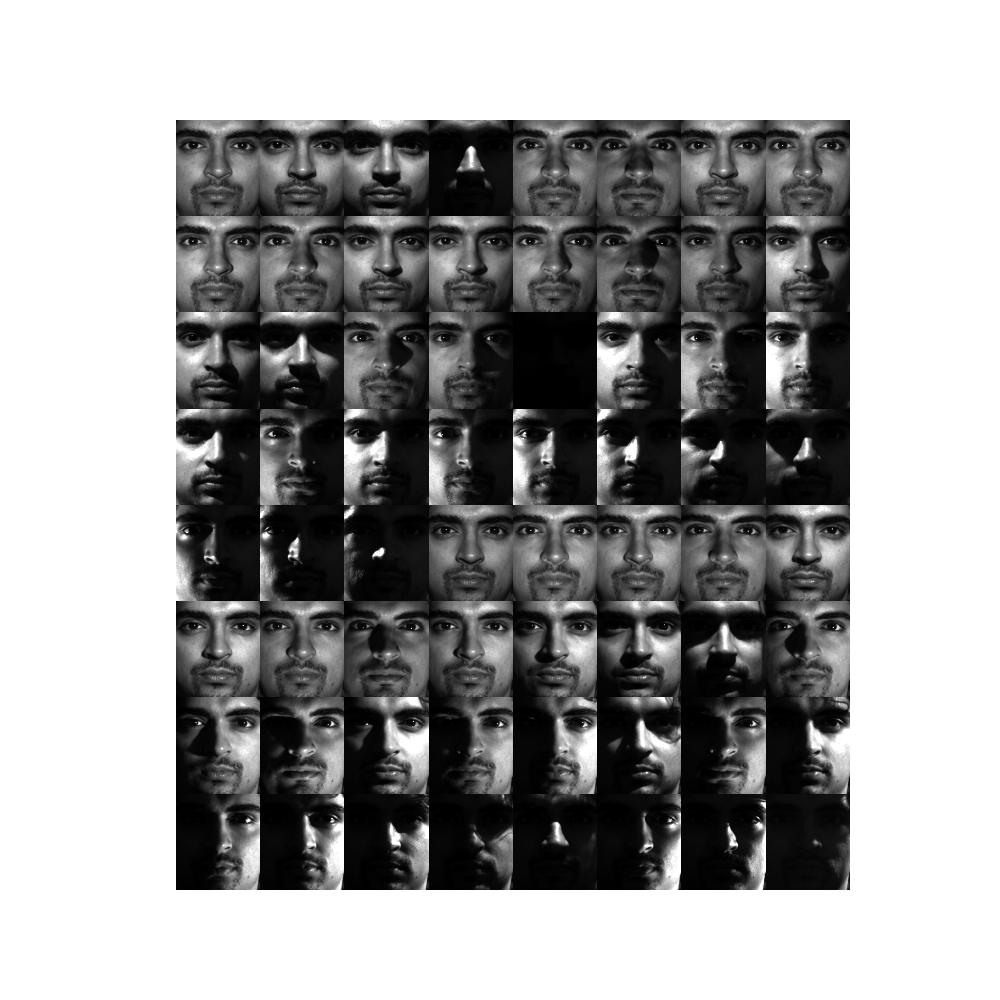
\includegraphics[height=0.35\textheight]{../media/face-8.png}
                \caption{Face 8}
            \end{figure}
            \begin{figure}[H]
                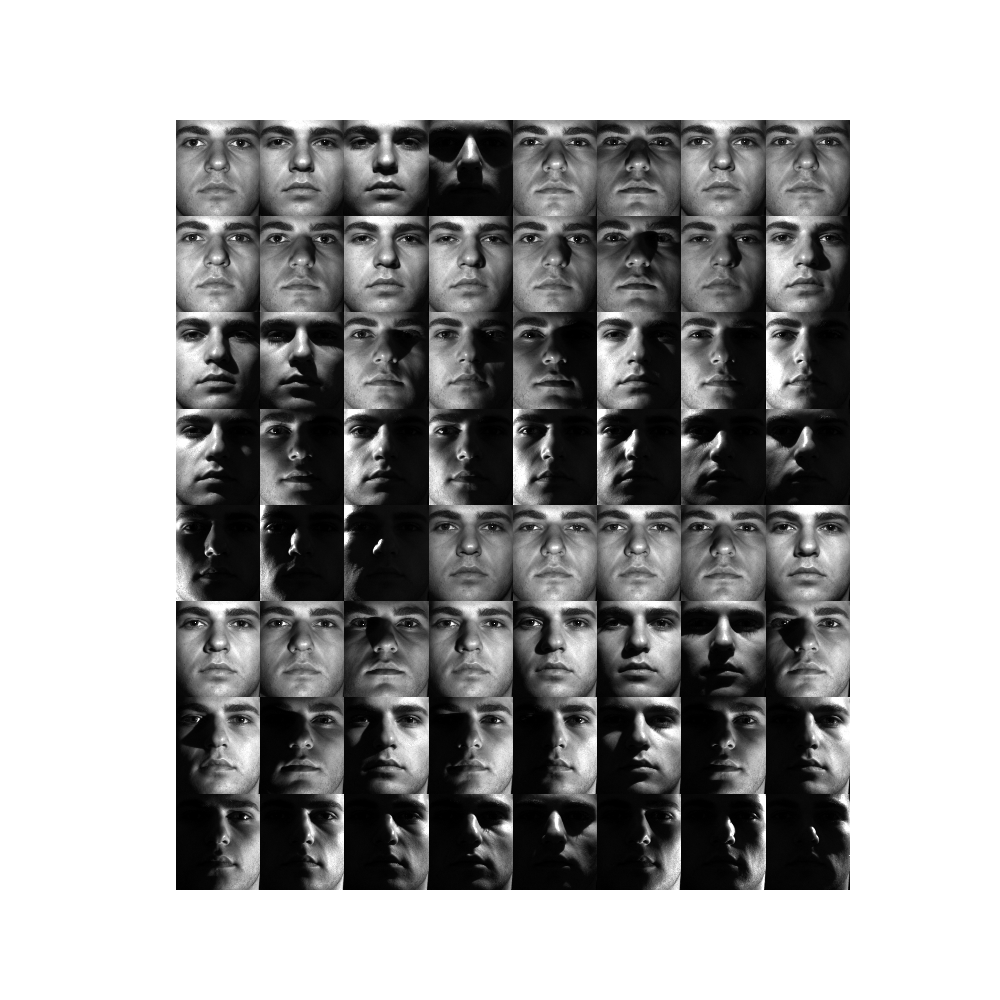
\includegraphics[height=0.35\textheight]{../media/face-24.png}
                \caption{Face 24}
            \end{figure}
        \end{mdframed}

    \item Next train the data by taking the SVD of the first 36 entries of
        the \texttt{faces} array subtracted by the mean of \texttt{faces}
        array. These values will correspond to the first 36 faces that we
        are training our data on. Verify you have completed this part
        correctly by comparing the images of the average face and the first
        column of $U$ to the provided figures. Once you have verified your
        code plot the 24\ts{th} mode of $U$ (i.e., $U[:,24]$).
        \begin{mdframed}[style=MyFrame]
            The 24\ts{th} mode of $U$ is shown below.
            \begin{figure}[H]
                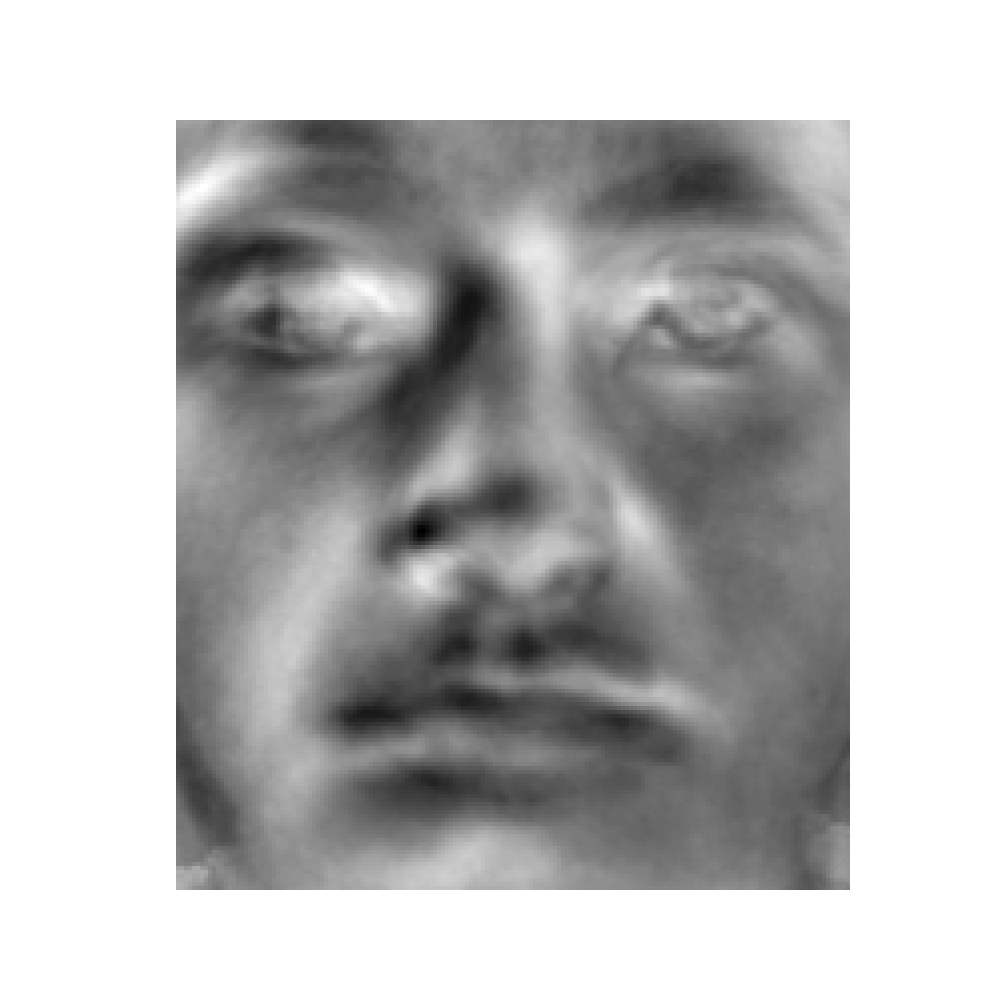
\includegraphics[height=0.35\textheight]{../media/mode-24.png}
                \caption{24\ts{th} mode of $U$}
            \end{figure}
        \end{mdframed}

    \item After confirming that the points have been trained correctly we
        can start attempting to reconstruct faces. Start by plotting and
        displaying face-37 and comparing that to the file provided. Next
        re-construct face-37 using the first 25, 50, 100, 200, 400, 800,
        and 1600 modes of $U$ and plotting your results. You should turn in
        8 plots for this task 1-original and 7-corresponding to the
        different modes. 
            \begin{mdframed}[style=MyFrame]
                Below are the plots for the corresponding modes.
                \begin{figure}[H]
                    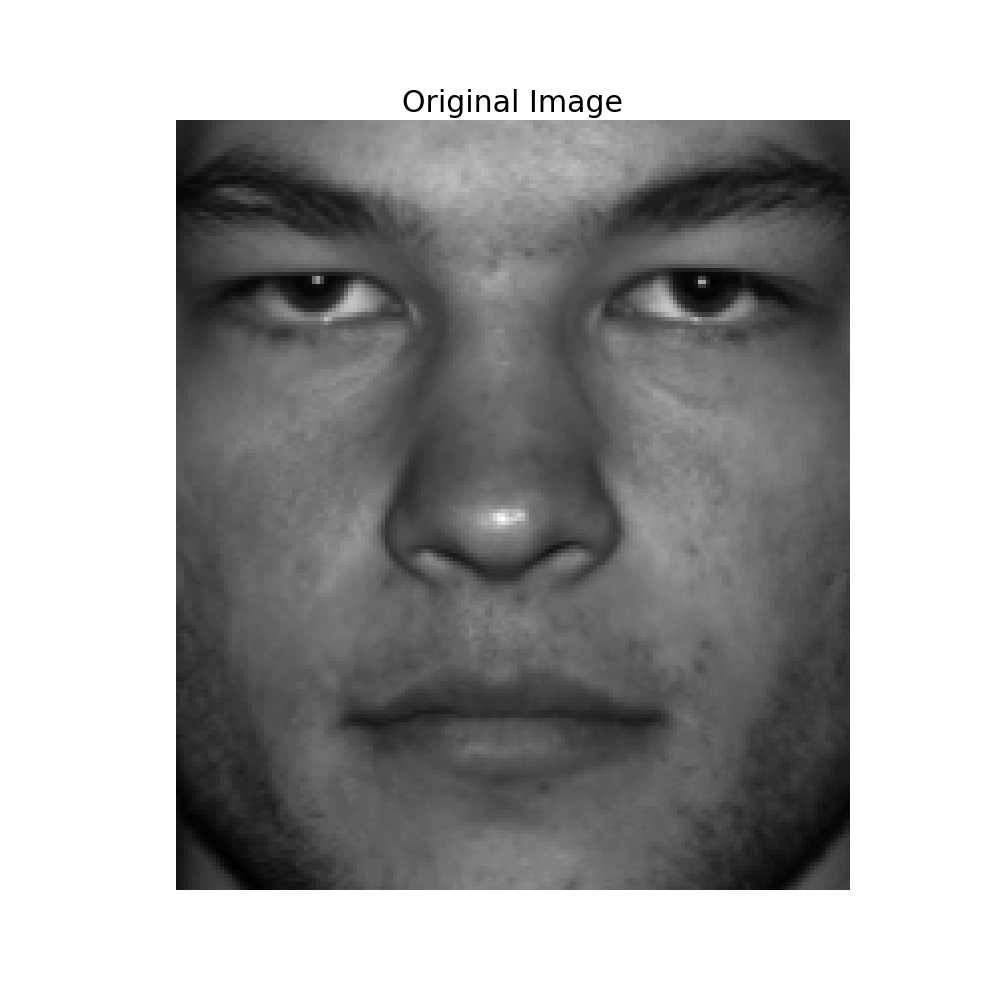
\includegraphics[height=0.35\textheight]{../media/original-image-1.png}
                    \caption{Face 37}
                \end{figure}
                \begin{figure}[H]
                    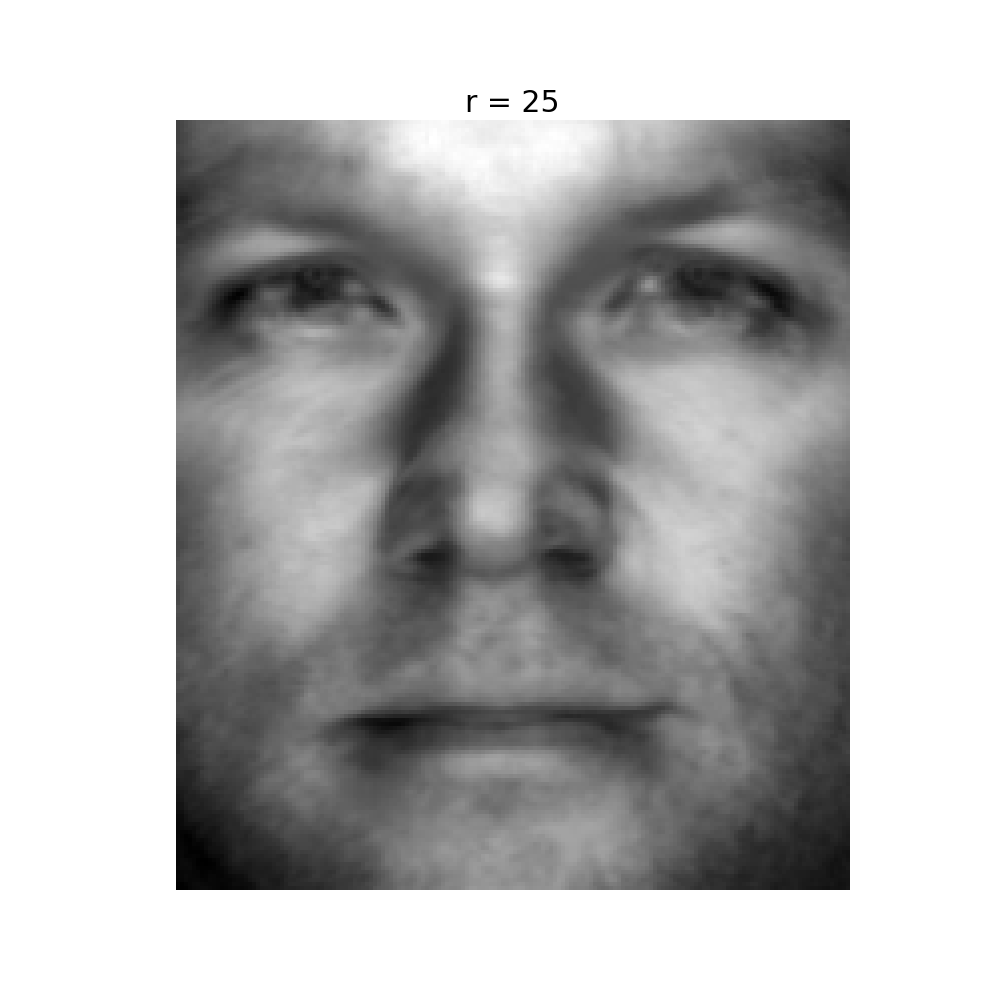
\includegraphics[height=0.35\textheight]{../media/r-25-1.png}
                    \caption{$r=25$}
                \end{figure}
                \begin{figure}[H]
                    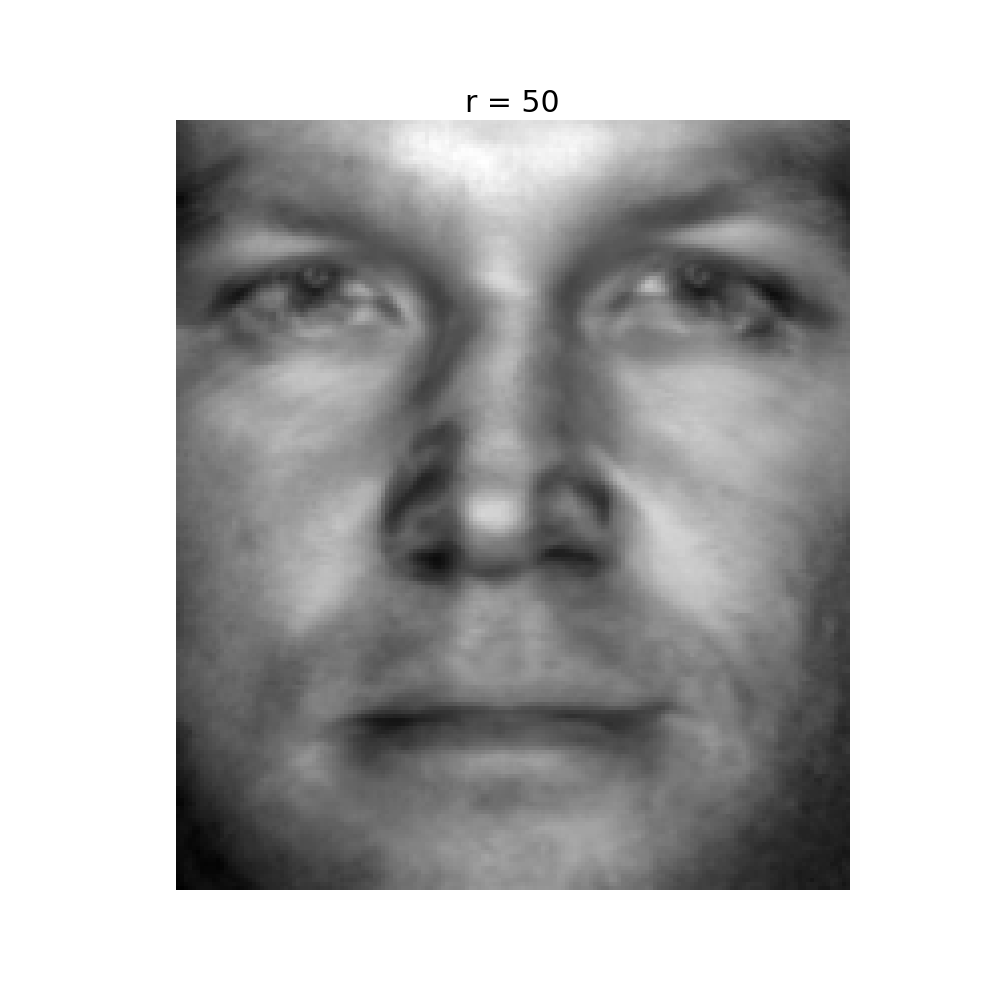
\includegraphics[height=0.35\textheight]{../media/r-50-1.png}
                    \caption{$r=50$}
                \end{figure}
                \begin{figure}[H]
                    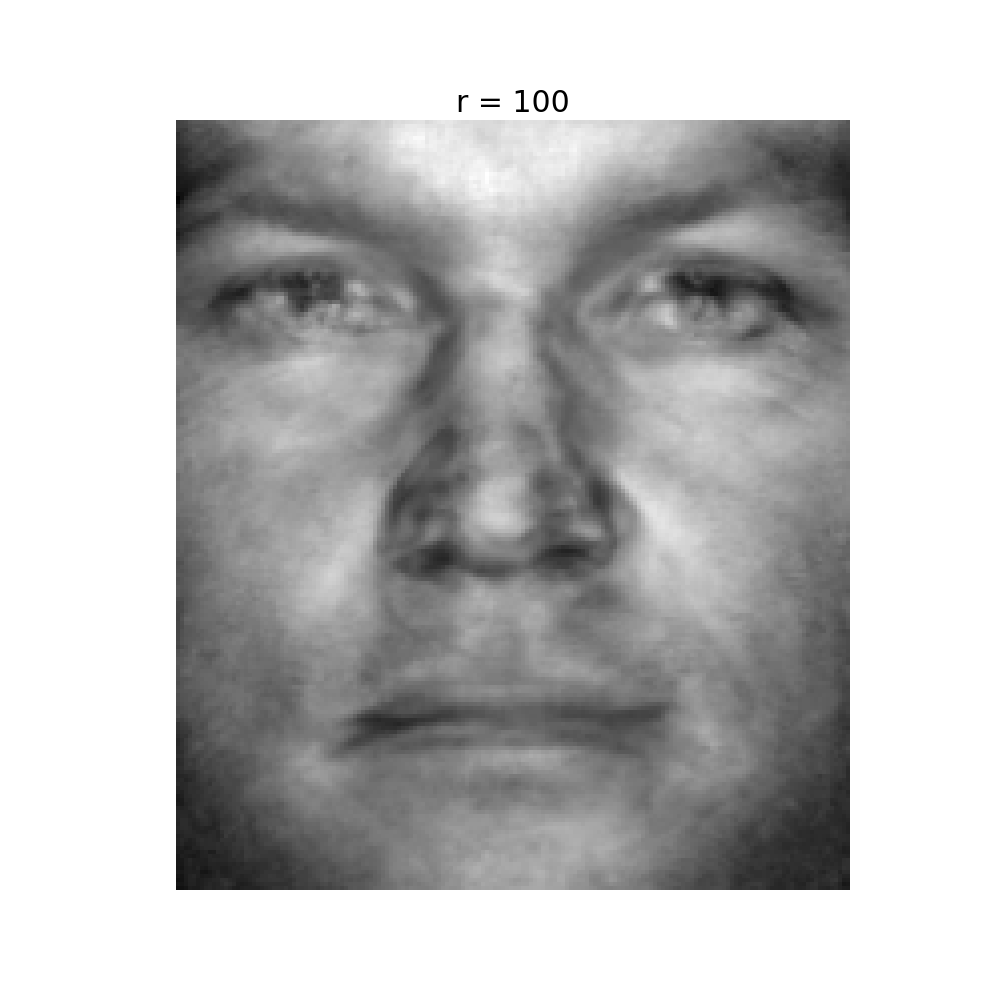
\includegraphics[height=0.35\textheight]{../media/r-100-1.png}
                    \caption{$r=100$}
                \end{figure}
                \begin{figure}[H]
                    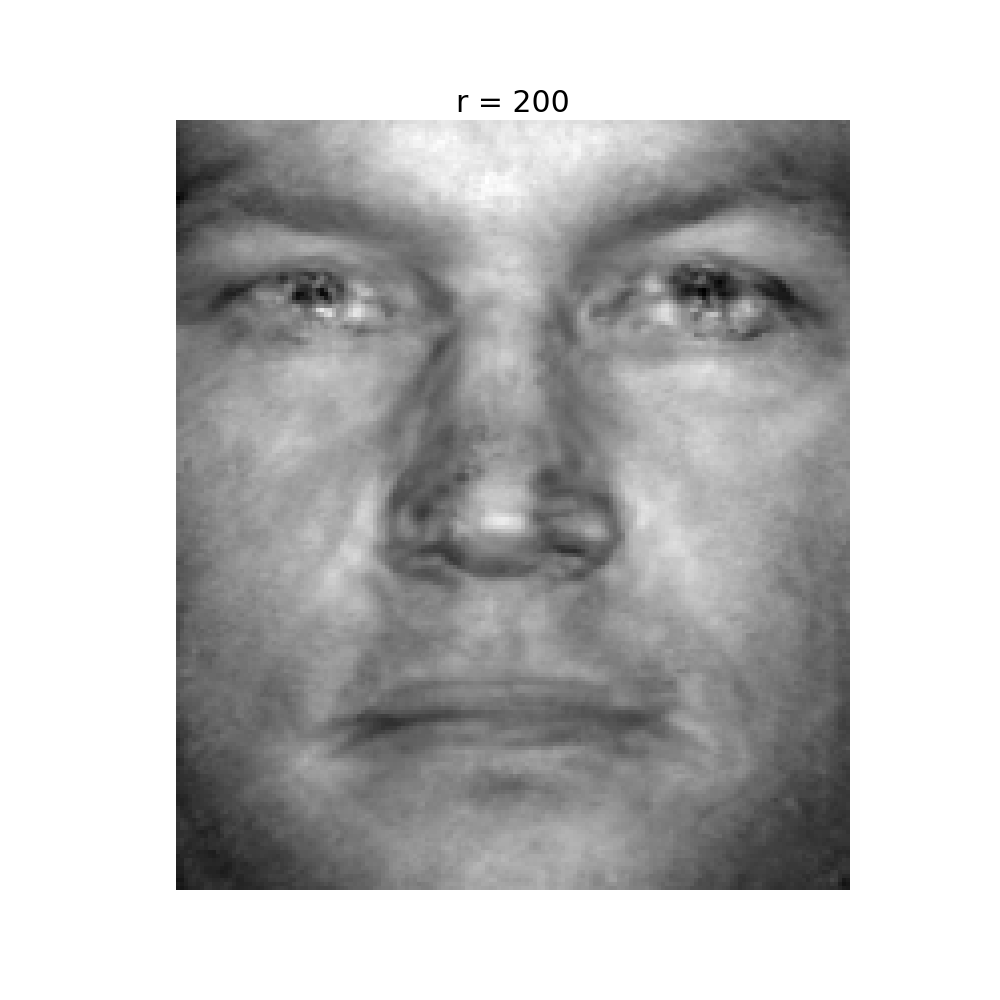
\includegraphics[height=0.35\textheight]{../media/r-200-1.png}
                    \caption{$r=200$}
                \end{figure}
                \begin{figure}[H]
                    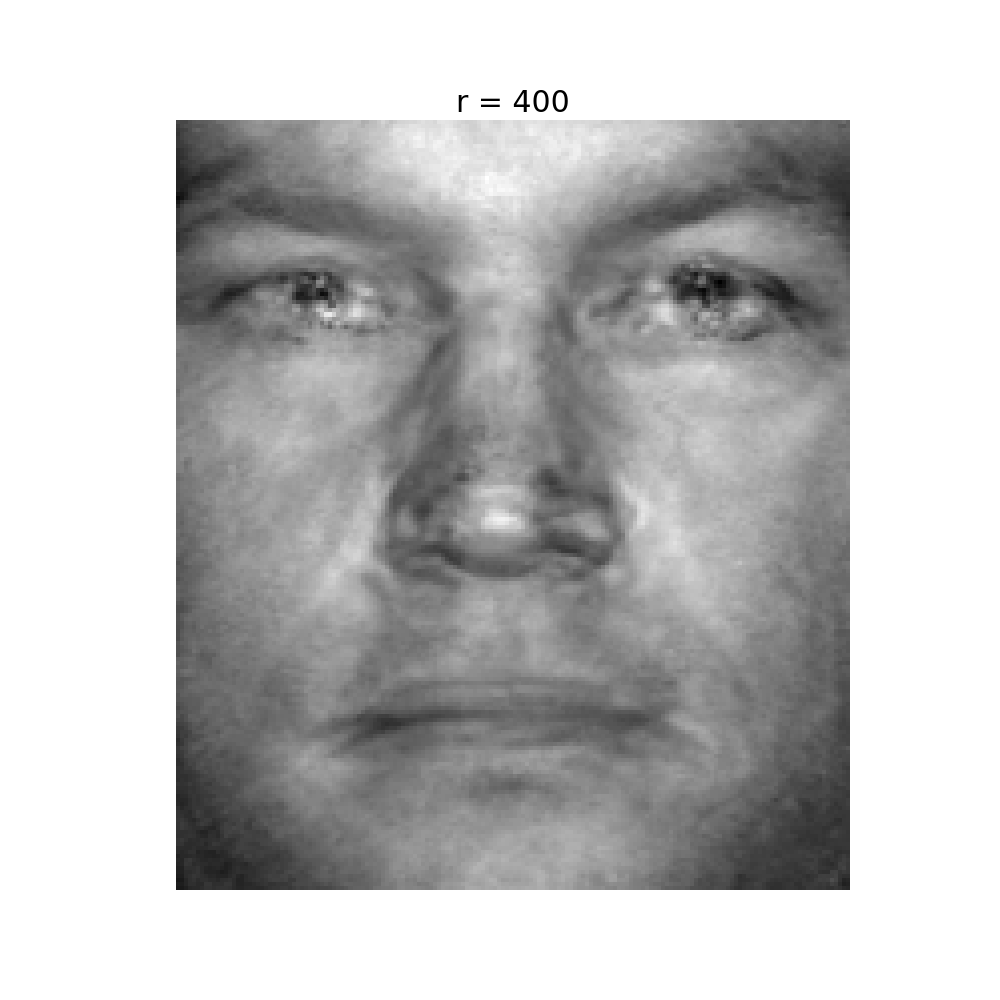
\includegraphics[height=0.35\textheight]{../media/r-400-1.png}
                    \caption{$r=400$}
                \end{figure}
                \begin{figure}[H]
                    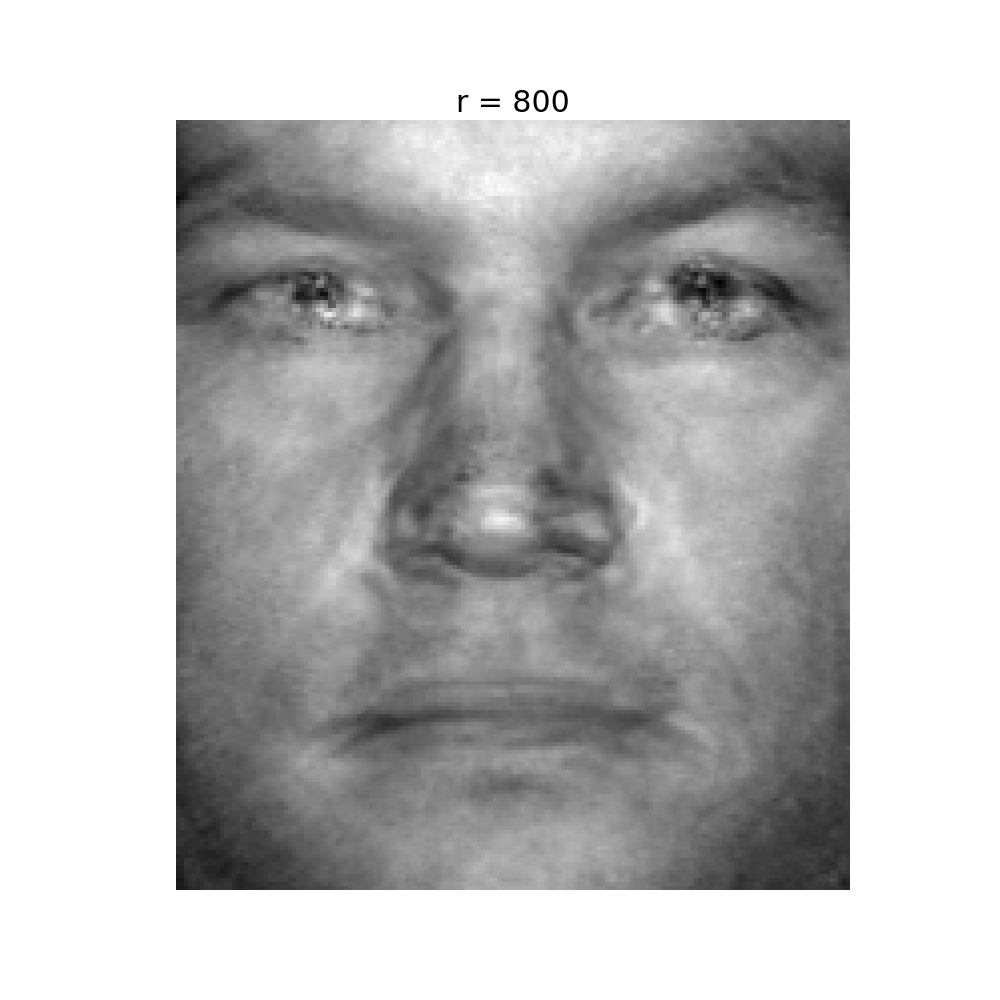
\includegraphics[height=0.35\textheight]{../media/r-800-1.png}
                    \caption{$r=800$}
                \end{figure}
                \begin{figure}[H]
                    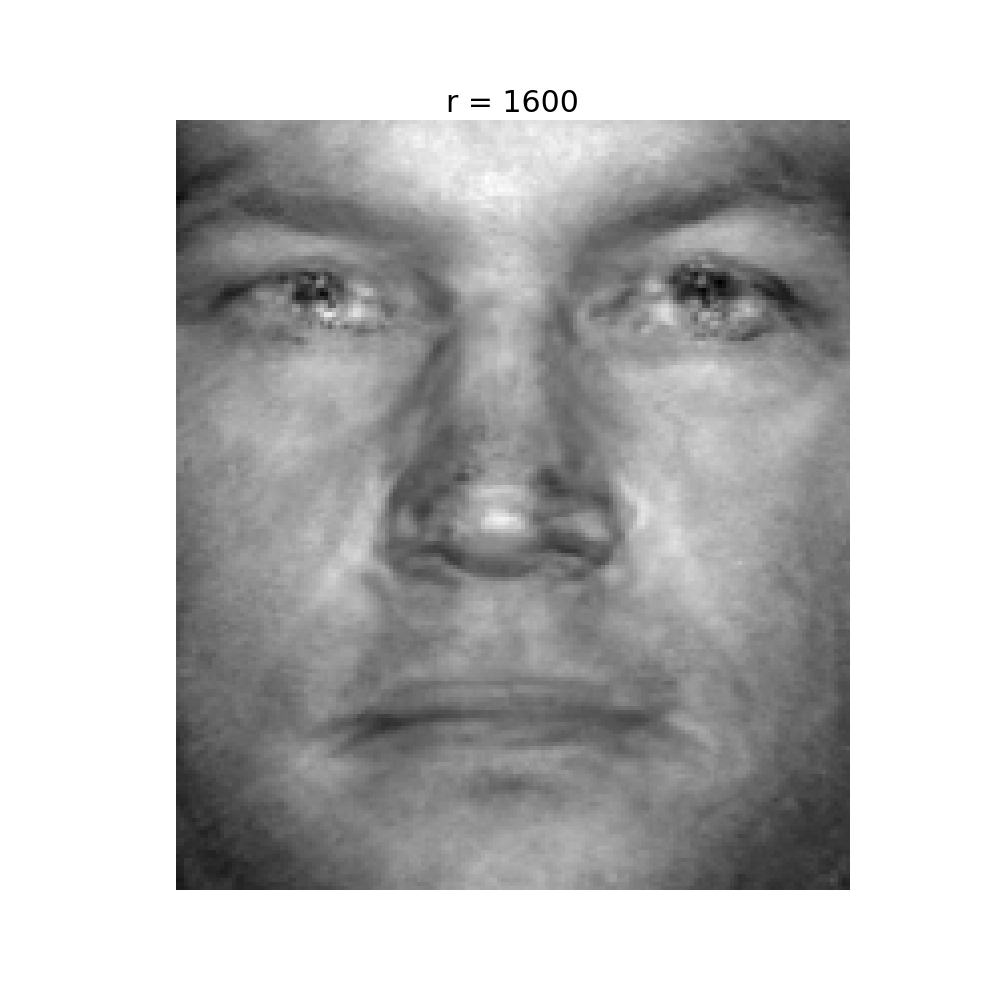
\includegraphics[height=0.35\textheight]{../media/r-1600-1.png}
                    \caption{$r=1600$}
                \end{figure}
            \end{mdframed}
    \item Repeat the above step for face-38 and plot the results, again
        there should be 8-plots.
            \begin{mdframed}[style=MyFrame]
                Below are the plots for the corresponding modes.
                \begin{figure}[H]
                    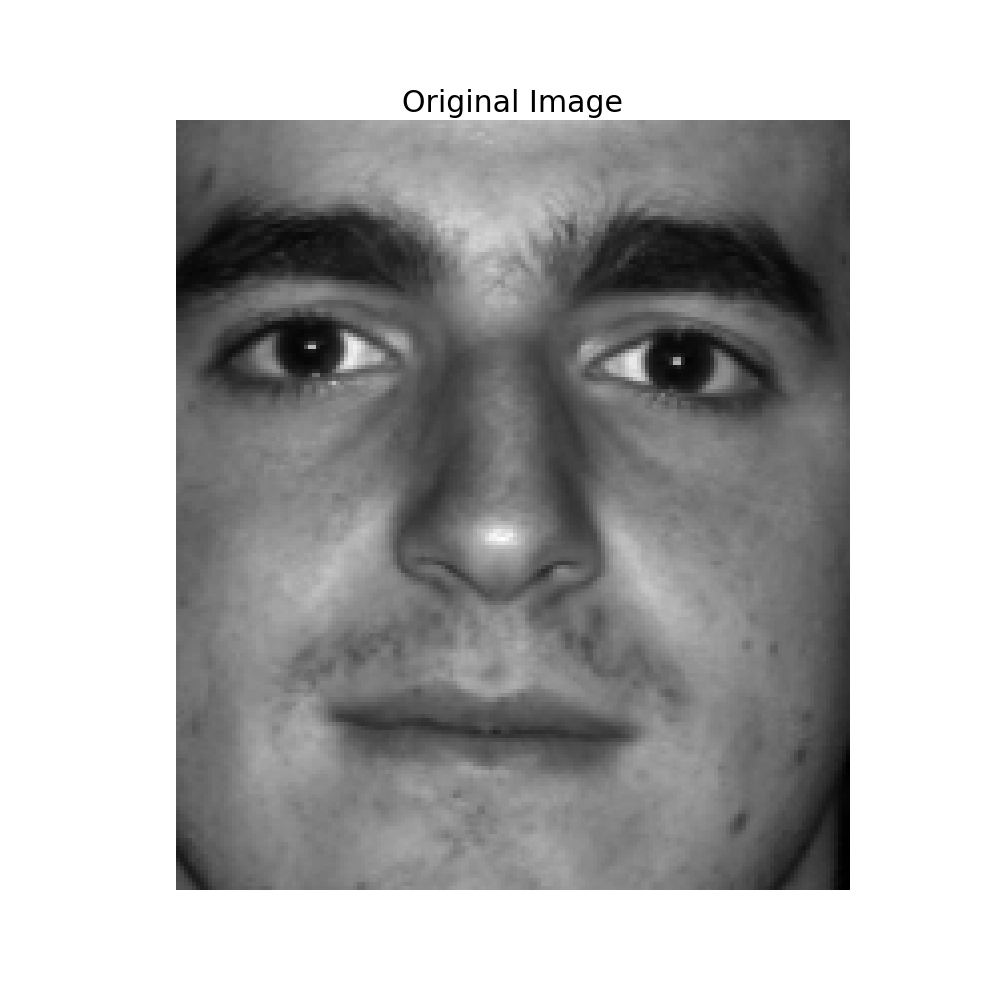
\includegraphics[height=0.35\textheight]{../media/original-image-2.png}
                    \caption{Face 37}
                \end{figure}
                \begin{figure}[H]
                    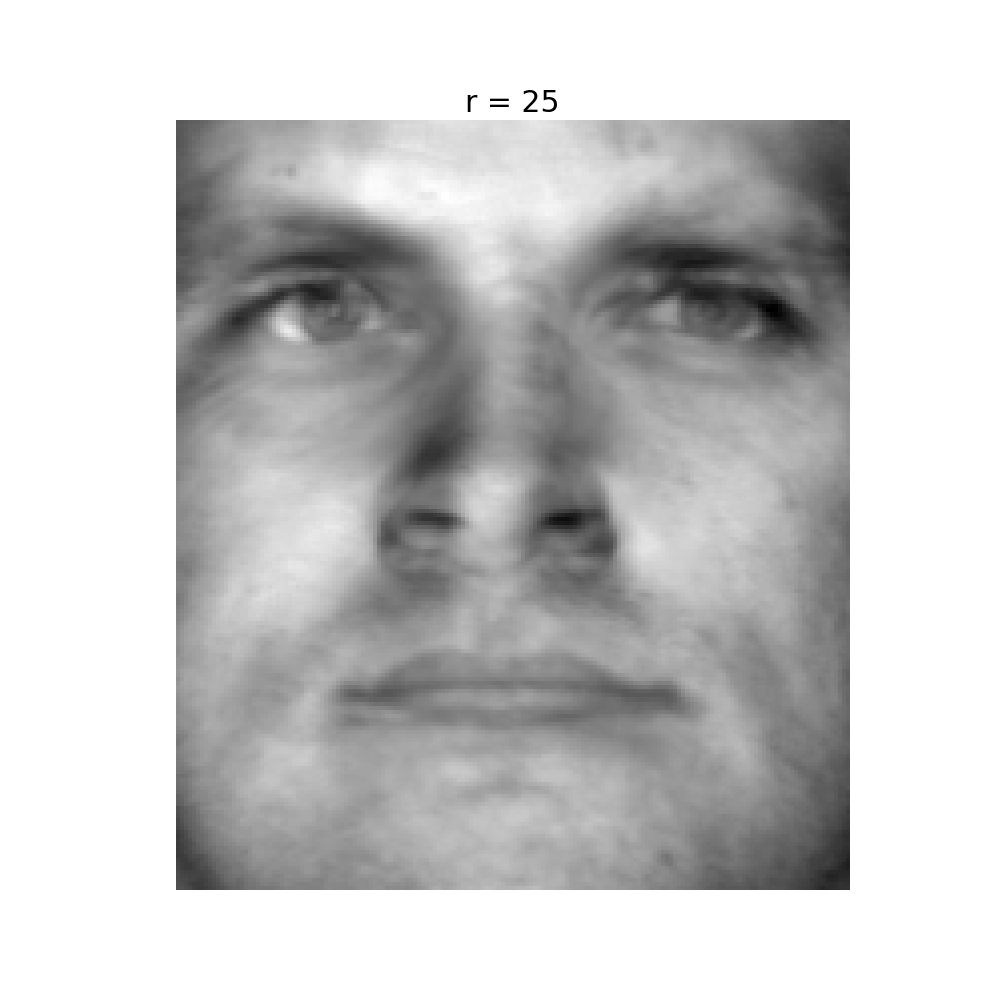
\includegraphics[height=0.35\textheight]{../media/r-25-2.png}
                    \caption{$r=25$}
                \end{figure}
                \begin{figure}[H]
                    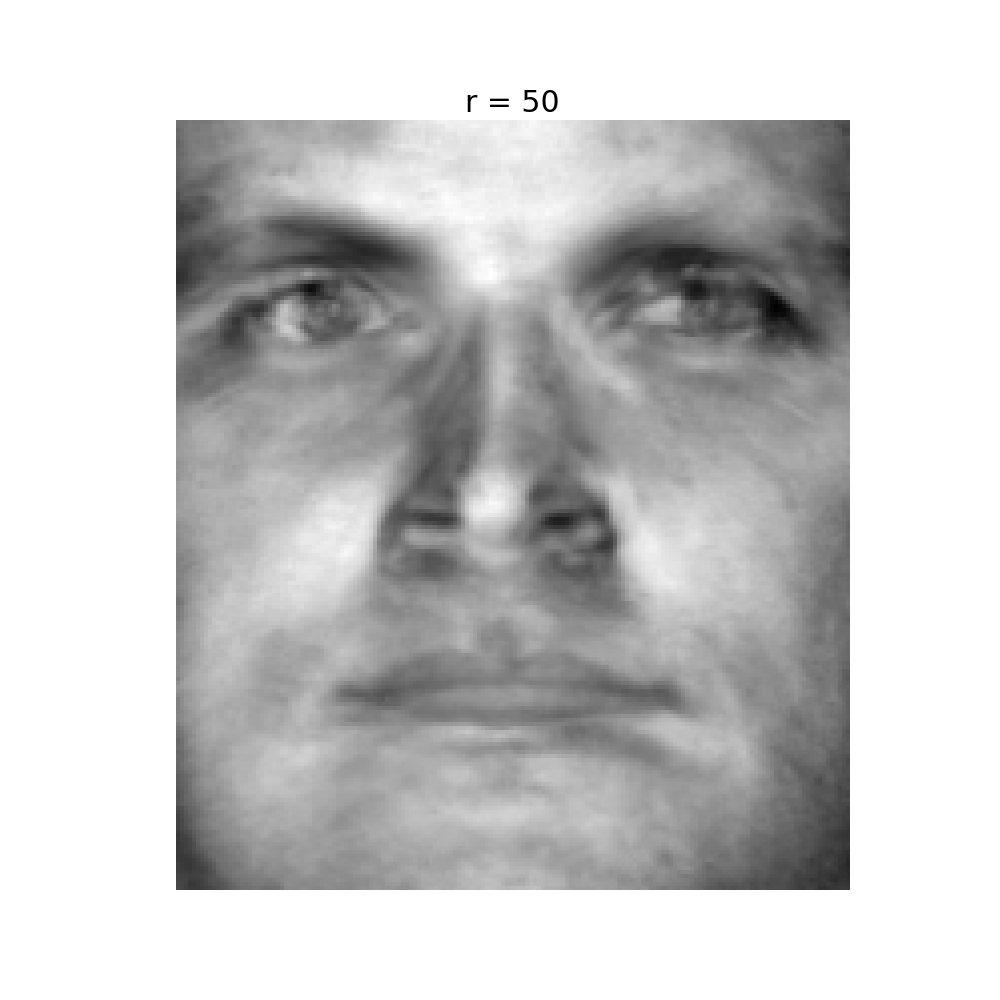
\includegraphics[height=0.35\textheight]{../media/r-50-2.png}
                    \caption{$r=50$}
                \end{figure}
                \begin{figure}[H]
                    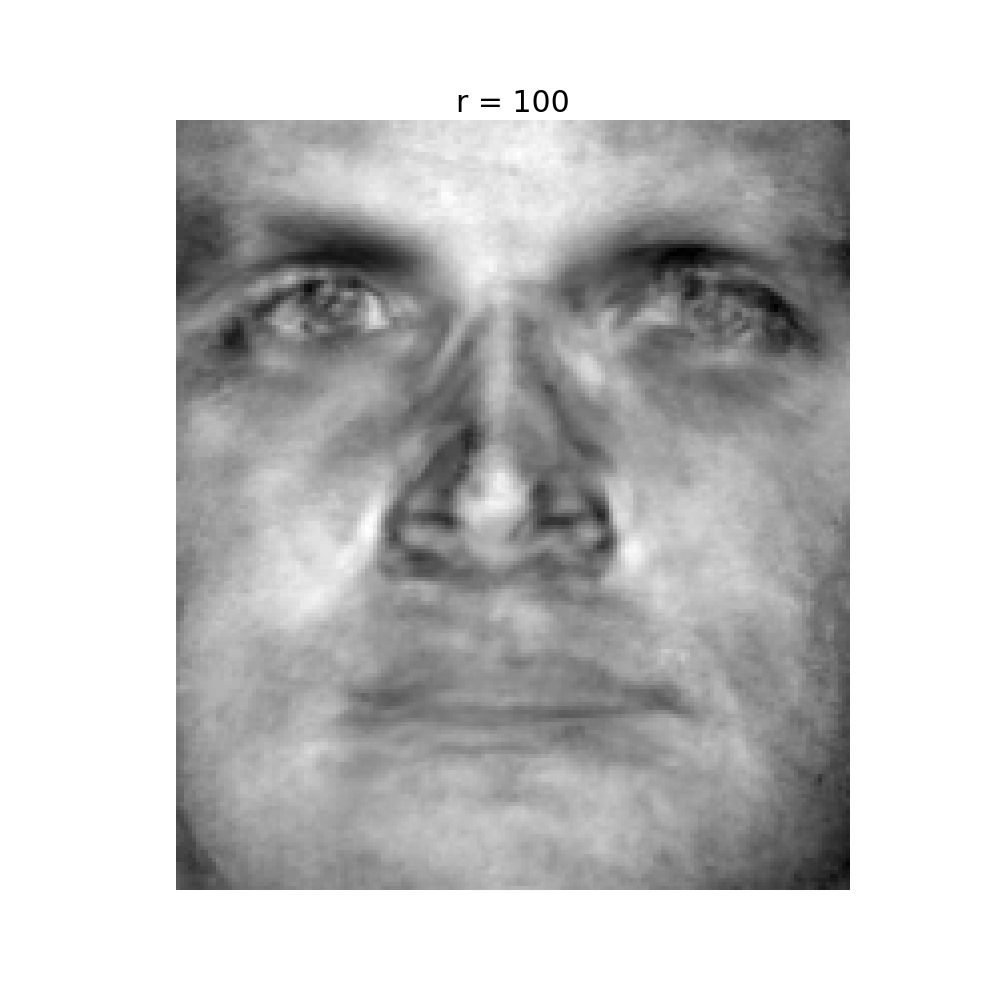
\includegraphics[height=0.35\textheight]{../media/r-100-2.png}
                    \caption{$r=100$}
                \end{figure}
                \begin{figure}[H]
                    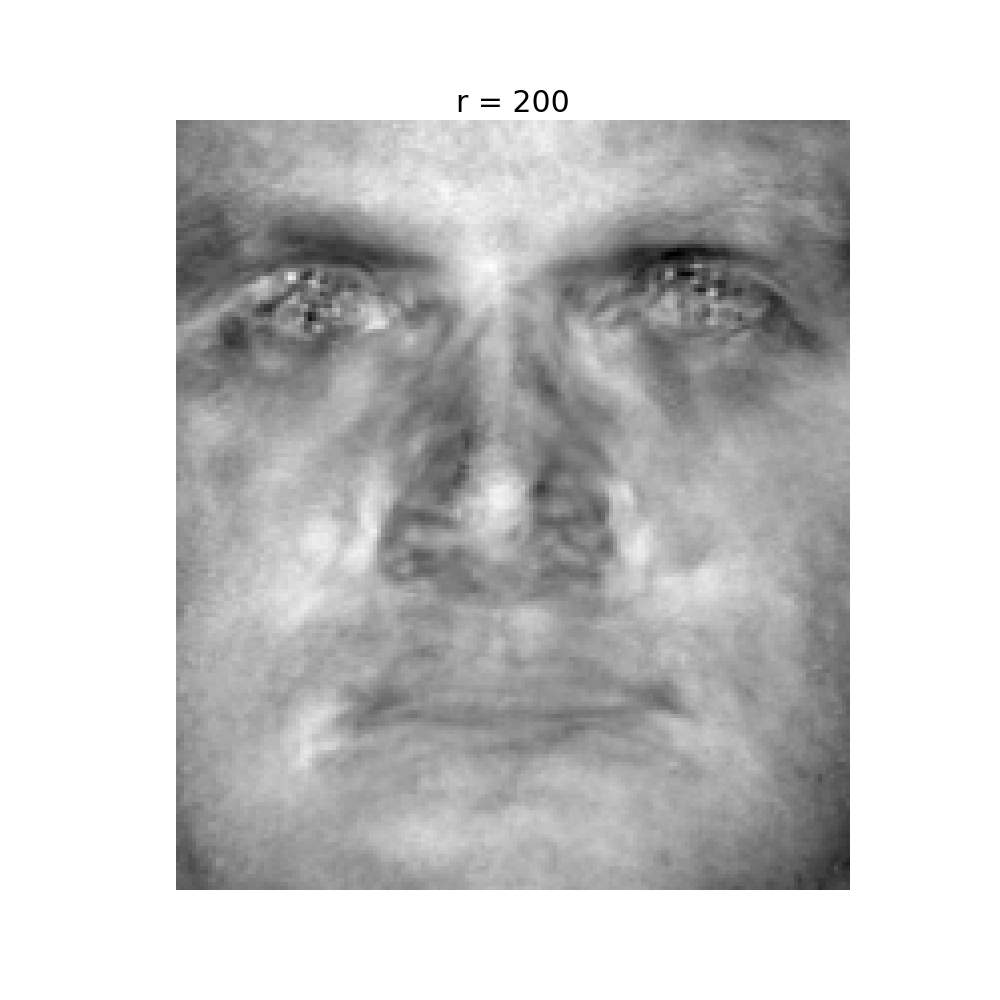
\includegraphics[height=0.35\textheight]{../media/r-200-2.png}
                    \caption{$r=200$}
                \end{figure}
                \begin{figure}[H]
                    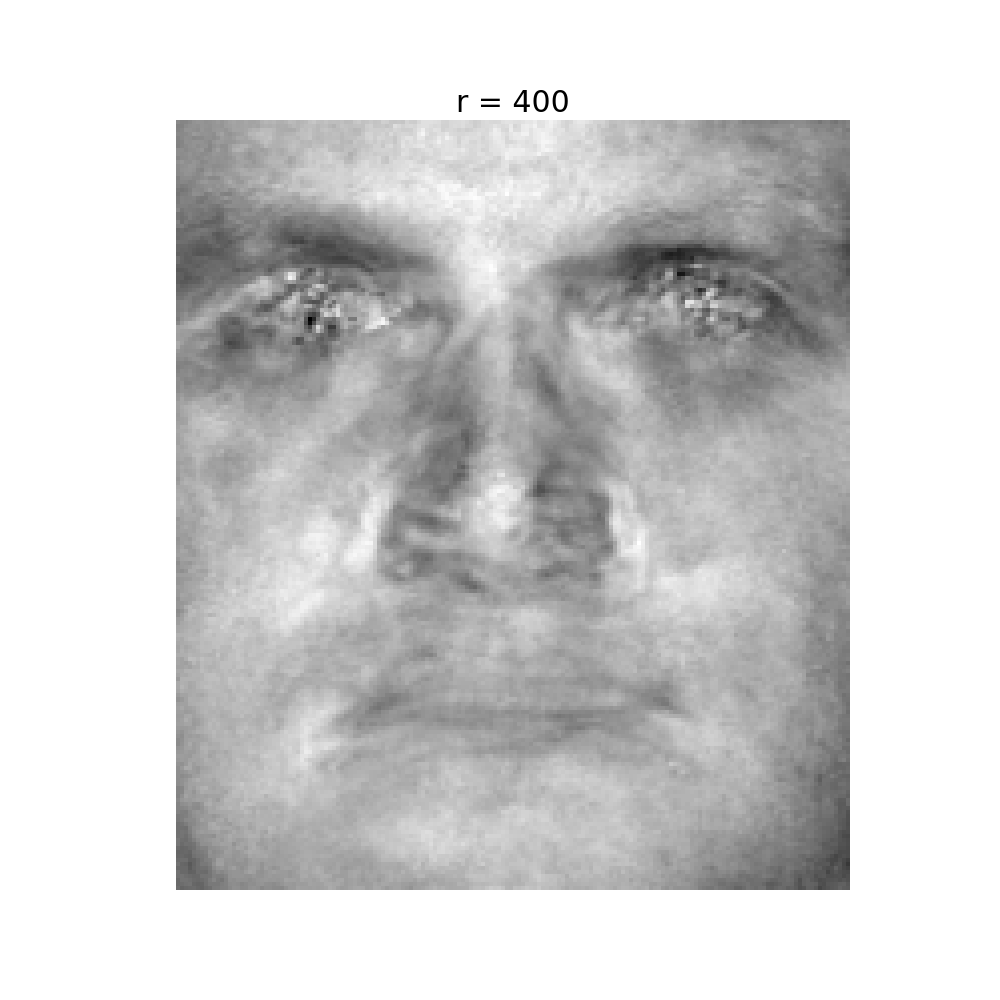
\includegraphics[height=0.35\textheight]{../media/r-400-2.png}
                    \caption{$r=400$}
                \end{figure}
                \begin{figure}[H]
                    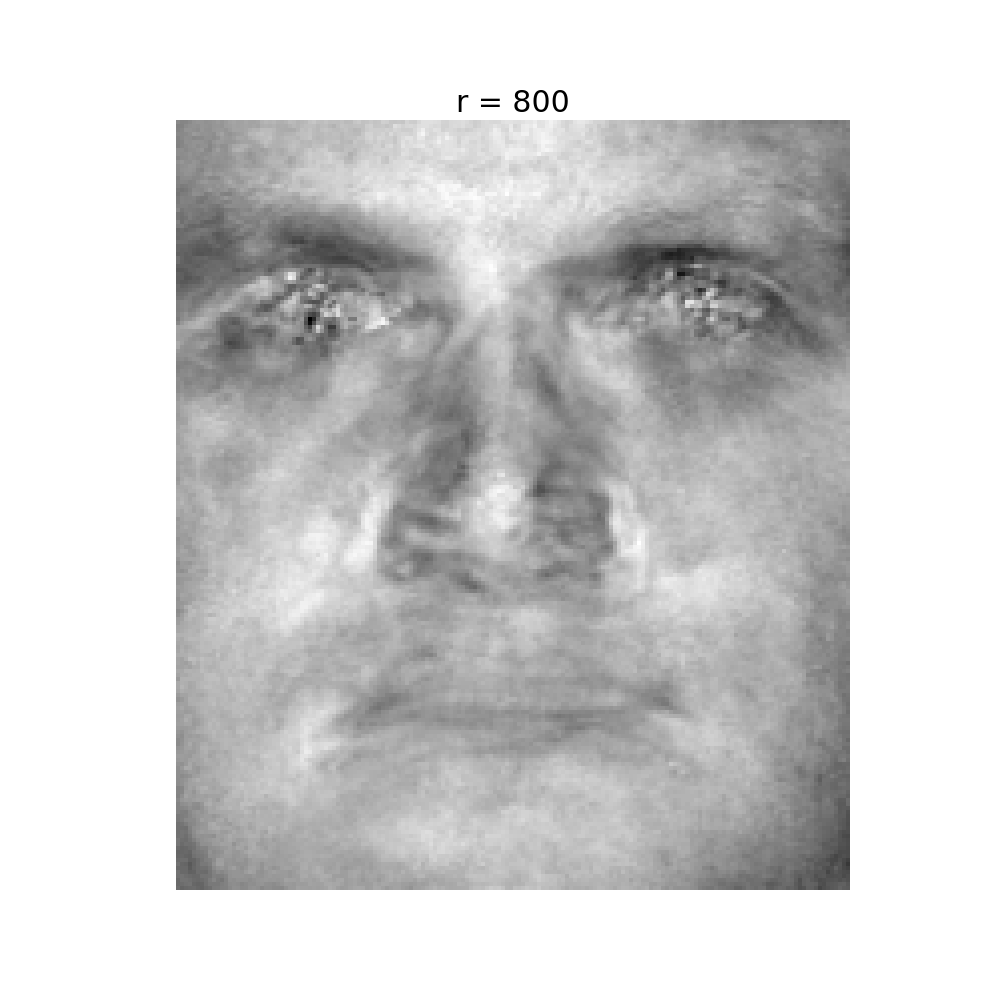
\includegraphics[height=0.35\textheight]{../media/r-800-2.png}
                    \caption{$r=800$}
                \end{figure}
                \begin{figure}[H]
                    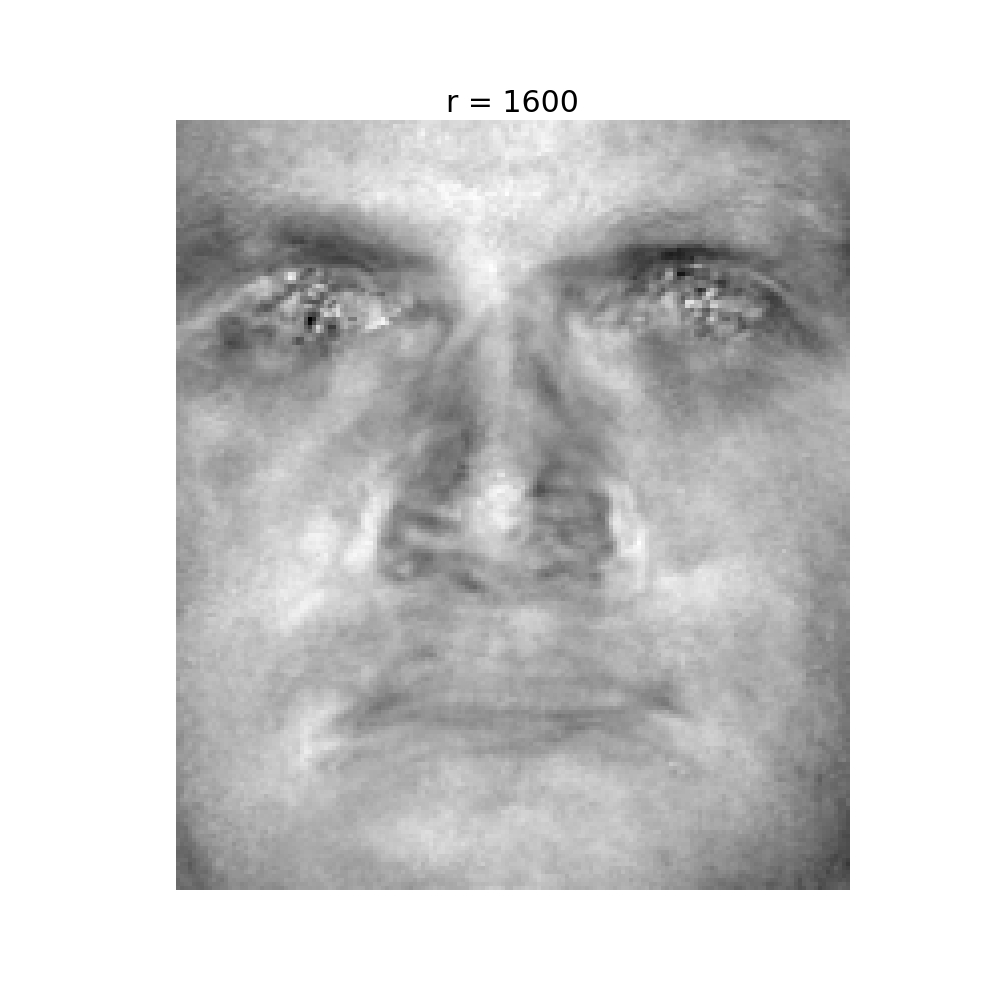
\includegraphics[height=0.35\textheight]{../media/r-1600-2.png}
                    \caption{$r=1600$}
                \end{figure}
            \end{mdframed}
\end{enumerate}
